%======================================================================
\chapter{Proces Twórczy}
%======================================================================

Każdy projekt indie zaczyna się od pomysłu, który wygląda lepiej w głowie niż w kodzie. Mój nie był wyjątkiem. W tym rozdziale piszę o tym, co zostało po roku iterowania - jak ze szkicu wyłonił się świat \textit{Echoes of Vanitas}, dlaczego główny bohater jest akurat nietoperzem, oraz co z pierwotnego planu udało się dowieźć, a co zostało świadomie przesunięte na później.

\section{Zarys Fabuły}
%----------------------------------------------------------------------

Akcja gry toczy się w alternatywnym, średniowiecznym świecie zamieszkałym wyłącznie przez inteligentne zwierzęta. Świat ma własną historię i własne hierarchie społeczne. Ludzie dawno wymarli, a pamięć o nich stała się tabu albo legendą - w zależności od tego, kto pyta.

Głównym bohaterem jest \textbf{Nietoperz Złodziej}. Samotnik, mieszkaniec skraju lasu, żyjący z drobnych kradzieży. Pewnego dnia natrafia na zakurzoną księgę spisaną w nieznanym języku. W miarę tłumaczenia odkrywa, że język ten należał do ludzi - rasy, której już nie ma. Wiedza zawarta w księdze niesie zarówno potencjał, jak i zagrożenie; każda decyzja gracza wpływa na to, w którą stronę pochyli się historia.

Z całej narracji w obecnej wersji zaimplementowałem jeden, ale za to kompletny wątek: quest główny \textit{Pętla Vanitas}. Jest to sekwencyjne zadanie wielokrokowe - zdobądź klucz (mini-gra w hubie), zejdź w głębię lochu, wydobądź relikt przy wyjściu i donieś wieść strażnikowi przy bramie. Każdy ukończony etap dopisuje wpis do dziennika, dzięki czemu gracz odbiera wątek narracyjnie, a nie tylko jako pasek postępu.

\section{Projekt Świata Gry}
%----------------------------------------------------------------------

Świat \textit{Echoes of Vanitas} zaprojektowałem jako szereg zróżnicowanych regionów. Poniżej zestawiam planowane lokacje z tym, co rzeczywiście trafiło do oddawanej wersji:

\begin{itemize}
    \item \textbf{Katakumby (hub)} [\textit{zrealizowane}] - lokacja startowa stanowiąca hub świata powierzchni. Mroczne korytarze z oświetleniem punktowym (zielone latarnie), kamienne ściany, skrzynie i beczki. Tu gracz rozmawia z NPC, przyjmuje quest i przechodzi przez bramę do proceduralnego lochu.
    \item \textbf{Proceduralny loch} [\textit{zrealizowane}] - drunkard's walk na siatce $9 \times 9$. Trzy warianty układu (różna liczba pokoi i kolory świateł), losowe modyfikatory runu, oświetlenie zależne od wariantu i modyfikatora \textit{Gloom}, spawny wrogów z jednolitym balansem HP/siły, elit i bossa w pokoju \texttt{Boss}, do trzech skrzyń, portal wyjścia w pokoju startowym. Klucz questowy z mini-gry w hubie; relikt przy pierwszym wyjściu. Dodatkowo: niewidzialni ujawniani radarem oraz minimapa w \texttt{SubViewport} z maską kołową.
    \item \textbf{Skraj lasu} [\textit{w planach}] - punkt startowy fabuły, dom bohatera.
    \item \textbf{Miasto zwierząt} [\textit{w planach}] - centrum handlowe i społeczne, NPC, handel.
    \item \textbf{Ruiny ludzkiej cywilizacji} [\textit{w planach}] - kluczowe dla wątku głównego.
    \item \textbf{Pałace monarchów} [\textit{w planach}] - strzeżone siedziby władców.
\end{itemize}

Środowisko katakumb zbudowane jest z modeli 3D renderowanych kamerą ortogonalną, co tworzy efekt 2.5D - bogatą oprawę wizualną przy zachowaniu płaskiej mechaniki ruchu. Loch współdzieli zestaw assetów z hubem, ale jego układ różni się dla każdej wyprawy dzięki proceduralnej generacji: wariant układu cyklicznie z liczby ukończonych runów, a ziarno losowe przy każdym wejściu.

\section{Koncepcje Postaci}
%----------------------------------------------------------------------

\subsection{Główny Bohater - Nietoperz Złodziej}

Projekt wizualny głównego bohatera łączy cechy charakterystyczne dla nietoperza (skrzydła jako płaszcz, duże uszy) z estetyką złodzieja-awanturnika. Postać przeszła kilka iteracji szkicowych zanim osiągnęła finalny wygląd.

\begin{figure}[htbp]
    \centering
    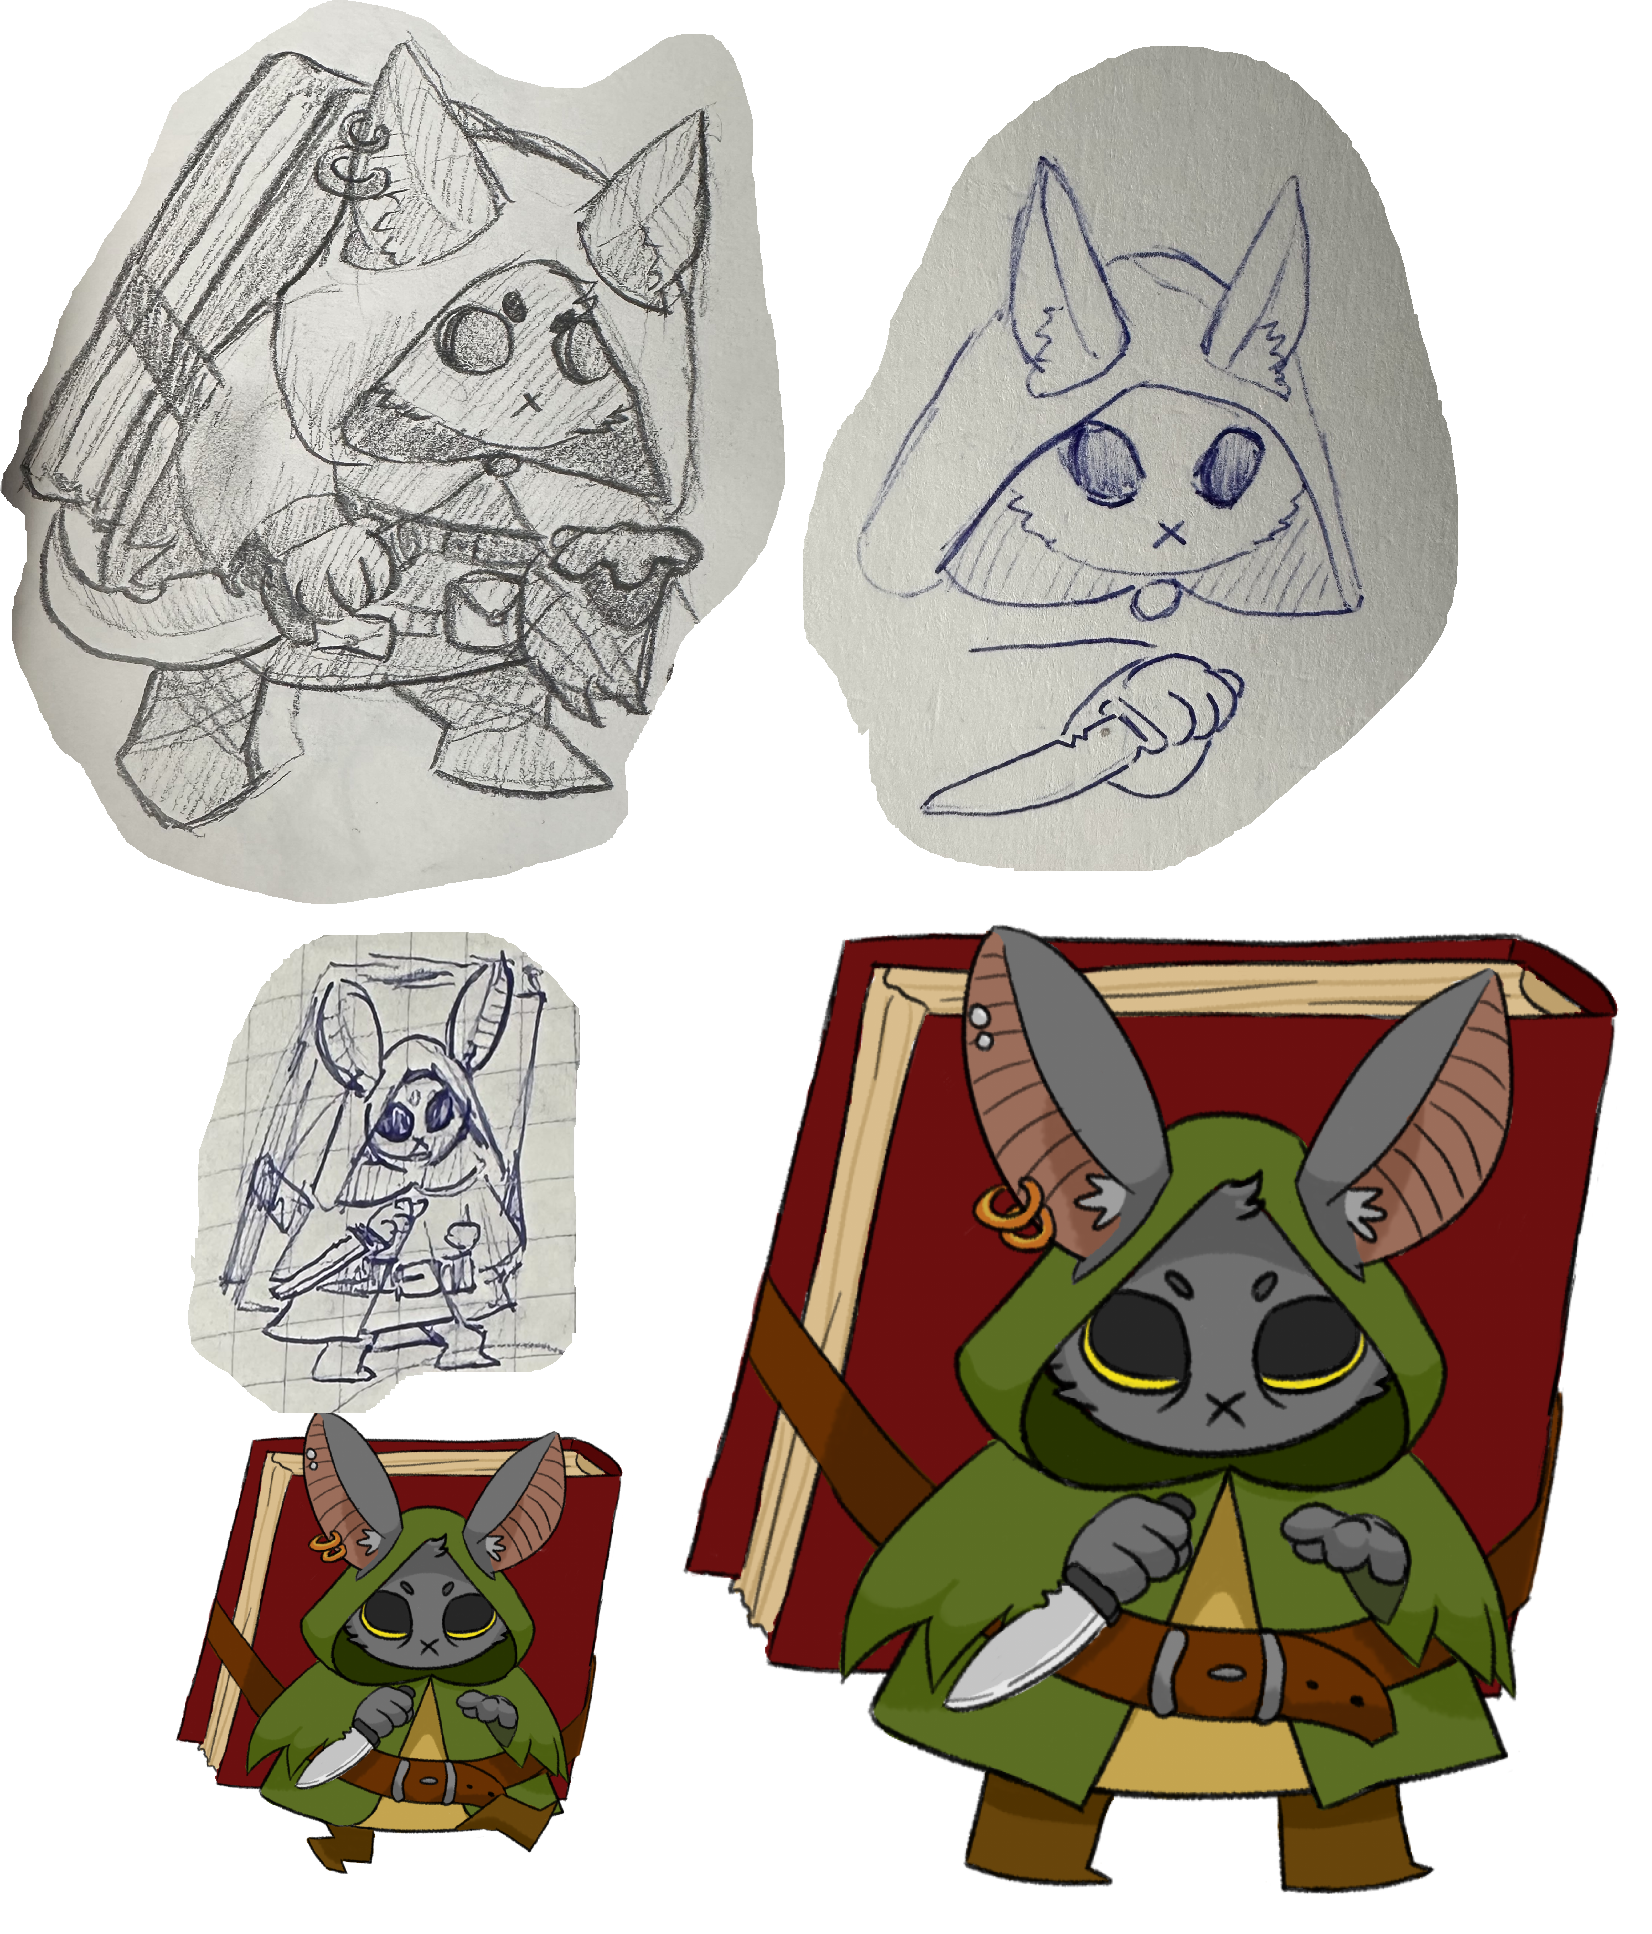
\includegraphics[width=0.75\textwidth]{images/bat-design.png}
    \caption{Źródło własne: Wczesne szkice koncepcyjne i finalny design Nietoperza Złodzieja. Clip Studio Paint.}
    \label{fig:bat-design}
\end{figure}

Bohater posiada statystyki: zdrowie (\textit{Health}), siłę (\textit{Strength}), złoto (\textit{Gold}) i doświadczenie (\textit{Experience}). Może być wyposażony w przedmioty z pięciu slotów: hełm, naszyjnik, sztylet, buty i strona (zwój). Każdy wyposażony przedmiot może być ulepszony (do maksymalnego poziomu \texttt{+MaxUpgradeLevel}), co zwiększa jego bonusy do statystyk.

\subsection{NPC - Labrador Rycerz}

Zrealizowany NPC to strażnik przy wejściu do katakumb - Labrador Rycerz. Łączy cechy rasy Labrador Retriever z estetyką rycerza w zbroi gotycko-fantasy. Jego rola obejmuje przekazanie questa pobocznego (\textit{Clean the Storage} - pokonaj $N$ wrogów typu \texttt{Roach}) oraz questa głównego (\textit{Pętla Vanitas}) z opisem narracyjnym, portretem i nagrodą końcową.

\begin{figure}[htbp]
    \centering
    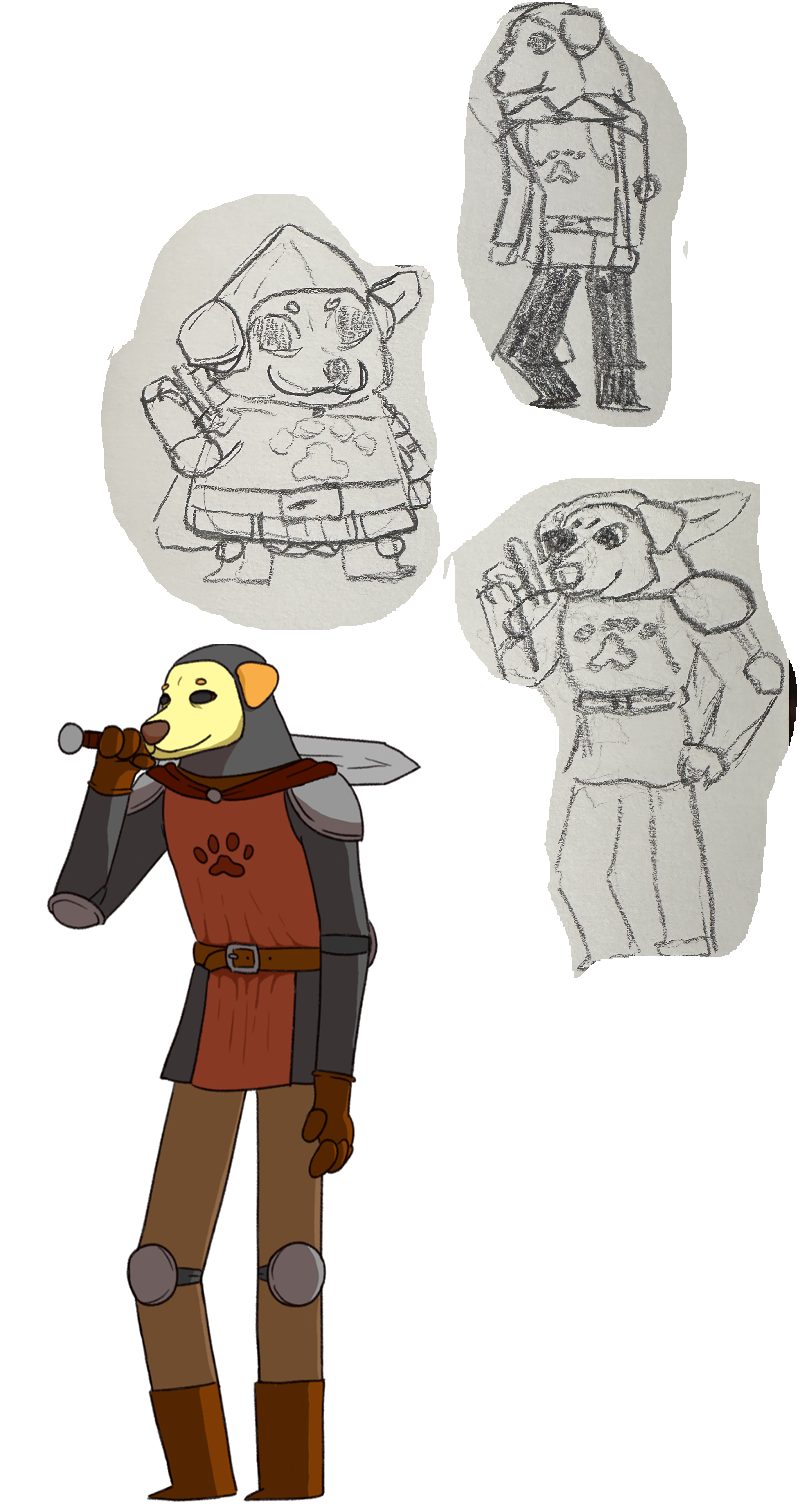
\includegraphics[width=0.75\textwidth]{images/labra_knight.png}
    \caption{Źródło własne: Szkice koncepcyjne i finalny design Labradora Rycerza. Clip Studio Paint.}
    \label{fig:labra-knight}
\end{figure}

\subsection{Przeciwnik - Insekt}

Bazowego przeciwnika zaprojektowałem jako antropomorficznego owada (rodzaj żuka/karalucha) o ptasiej, dziobatej głowie - sylwetka czytelna z lotu kamery, a zarazem trochę odrażająca, co pasuje do roli wroga. Ten sam zestaw sprite'ów obsługuje cztery warianty przeciwnika: zwykłego, elitę (fioletowy tint z shadera), bossa (powiększenie i czerwony tint) oraz niewidzialnego (sterowanie przezroczystością w kodzie) - dzięki temu jeden, dopracowany zestaw animacji wystarcza na całą menażerię. Rysunek~\ref{fig:enemy-sketch} pokazuje finalny projekt, szkice studyjne sylwetki oraz dobraną paletę kolorów.

\begin{figure}[htbp]
    \centering
    
\includegraphics[width=0.85\textwidth]{enemie_art_skeatch.png}
    \caption{Źródło własne: projekt przeciwnika-insekta - finalny design, szkice koncepcyjne sylwetki i paleta kolorów. Clip Studio Paint.}
    \label{fig:enemy-sketch}
\end{figure}

\subsection{Wstępny Zarys Stylu Postaci}

Poniższy rysunek przedstawia wstępny zarys postaci niegrywalnych w odniesieniu do planowanych lokacji. Jest to wczesna koncepcja projektowa, która posłużyła jako punkt wyjścia - większość tych postaci nie została jeszcze zaimplementowana.

\begin{figure}[htbp]
    \centering
    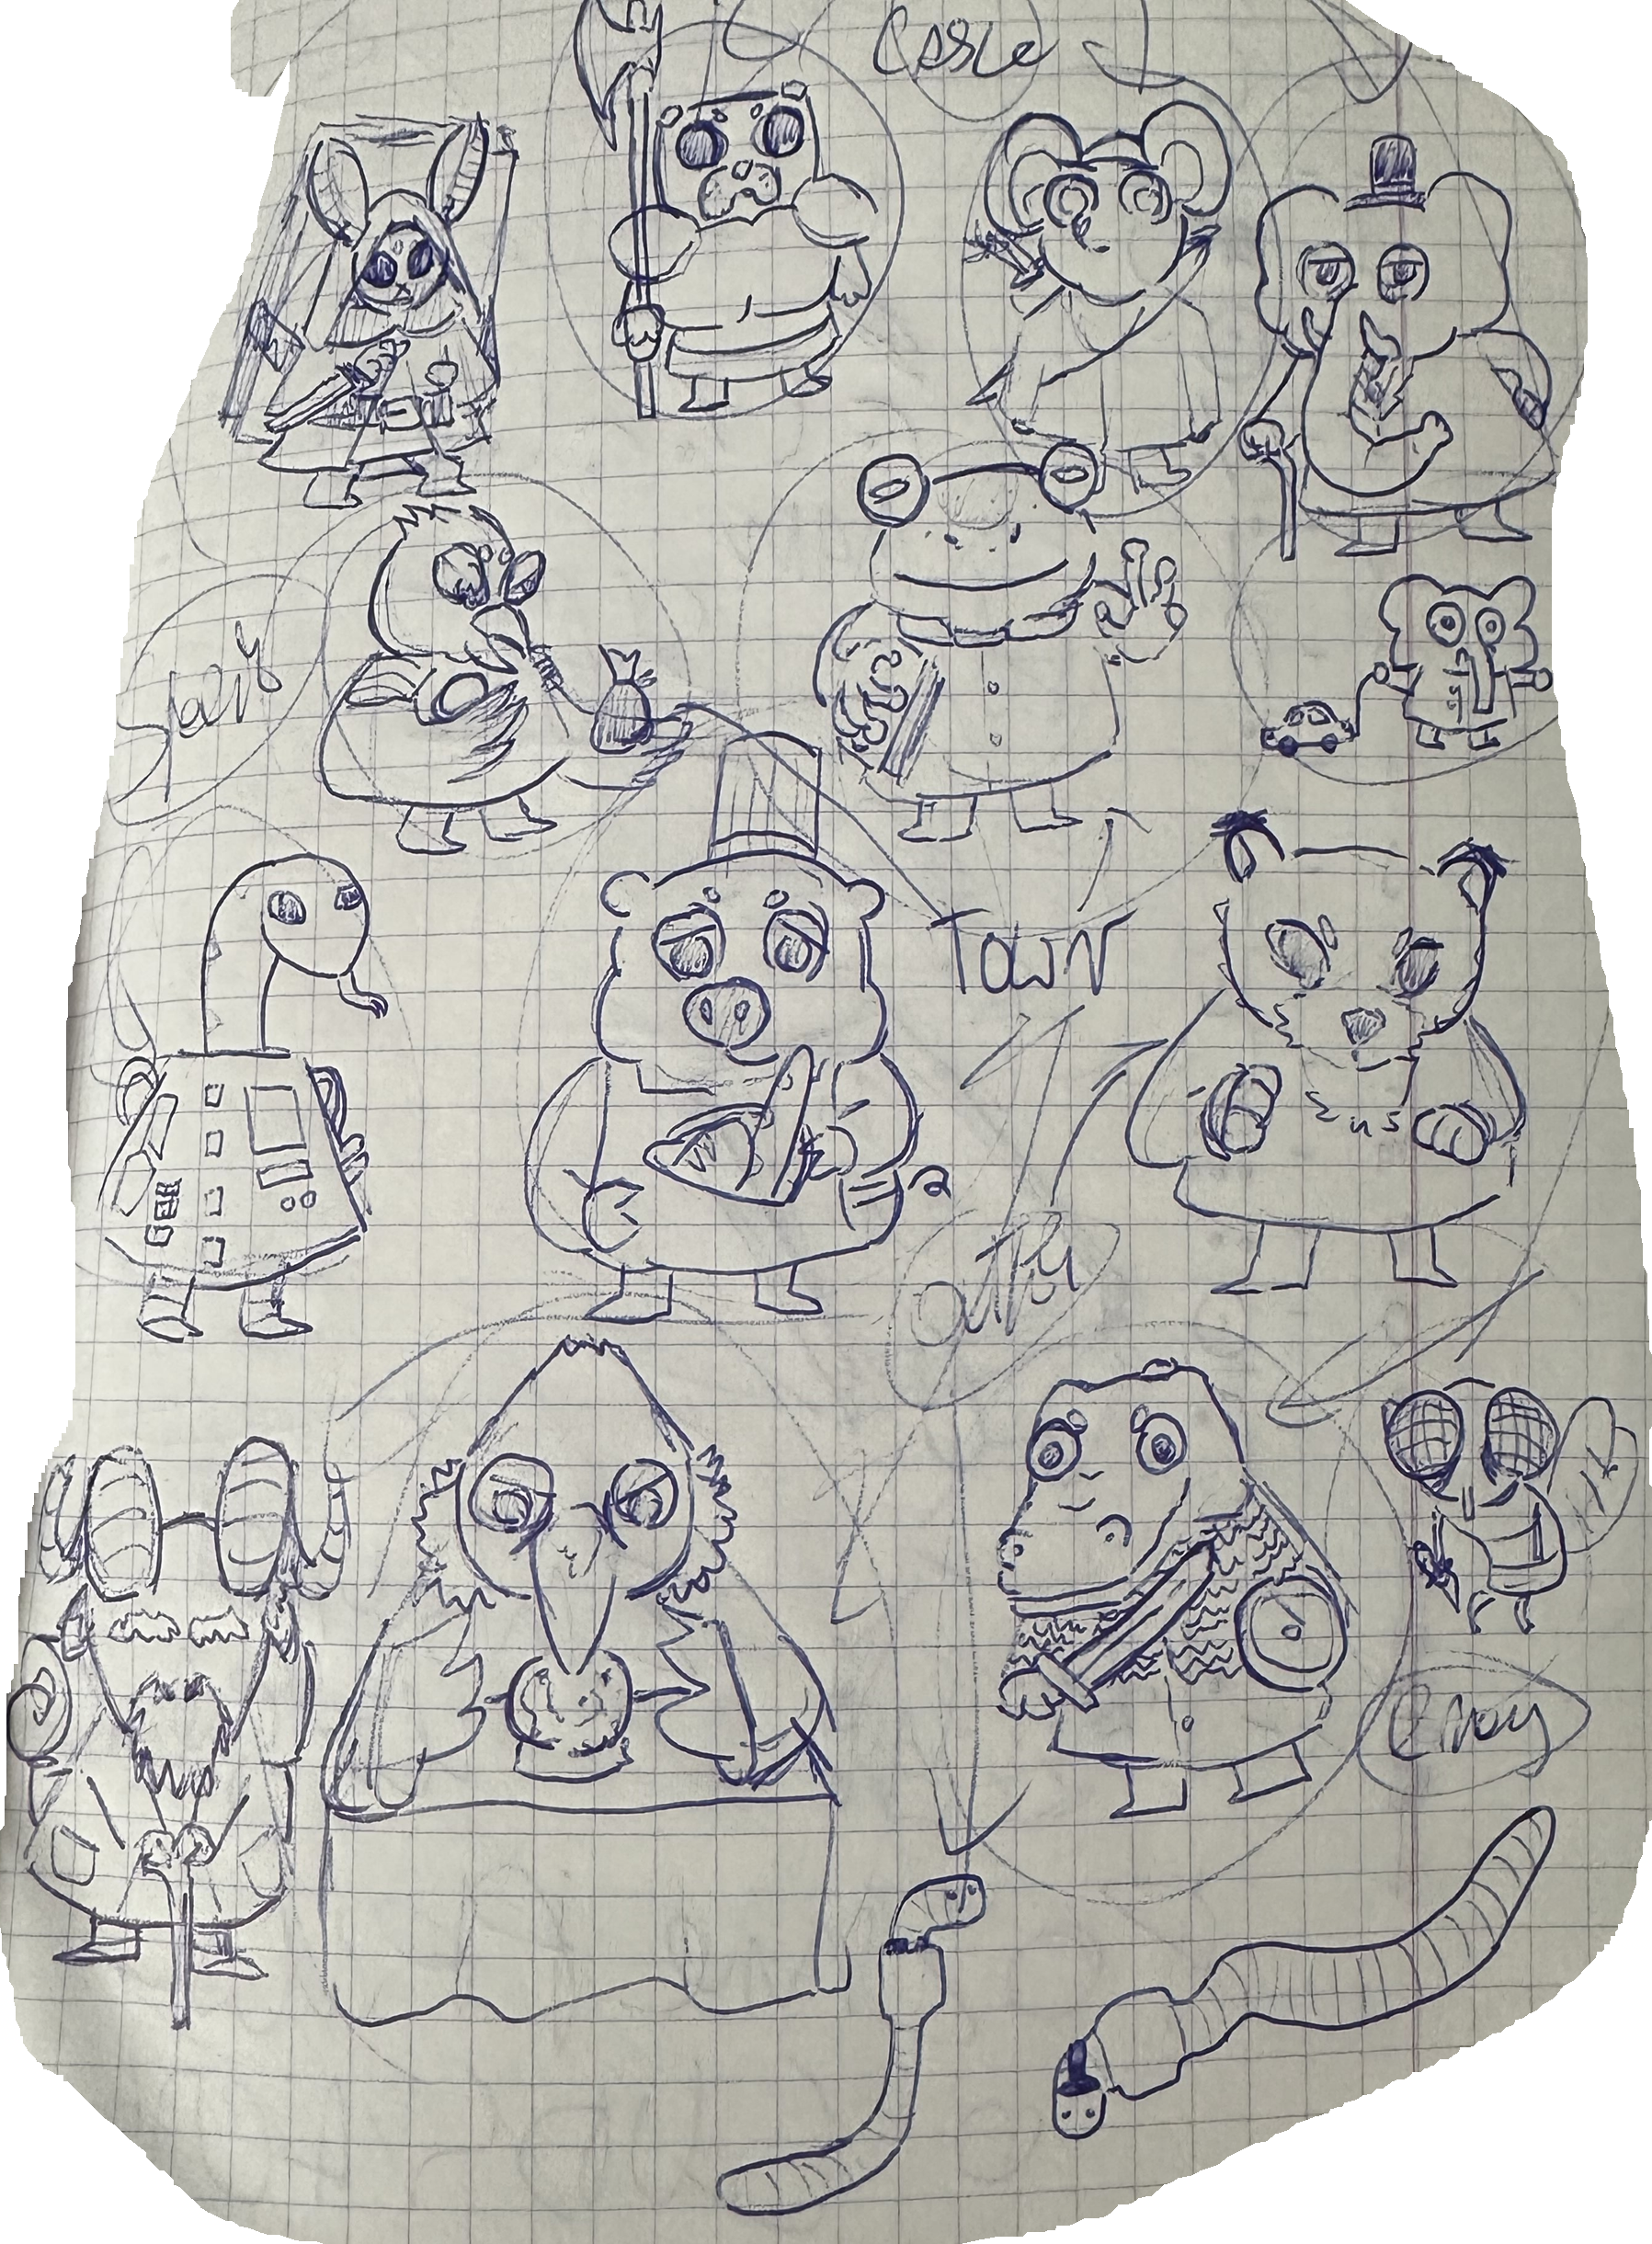
\includegraphics[width=0.75\textwidth]{images/npcs.png}
    \caption{Źródło własne: Wstępny szkic koncepcyjny postaci niegrywalnych.}
    \label{fig:npcs}
\end{figure}

\section{Decyzje Artystyczne}
%----------------------------------------------------------------------

\subsection{Styl Graficzny}

Całą warstwę graficzną gry narysowałem samodzielnie w programie Clip Studio Paint i traktuję ją jako jeden z głównych, autorskich wkładów tej pracy. Nie użyłem żadnych gotowych paczek sprite'ów, bibliotek ikon ani generatorów grafiki - każdy kadr postaci, każdy portret NPC i każda ikona ekwipunku powstały od pustego płótna.

Proces przy każdej postaci wyglądał podobnie: zaczynałem od kilku szkiców koncepcyjnych badających sylwetkę i charakter, wybierałem jeden kierunek, a następnie doprowadzałem go do finalnego, pokolorowanego sprite'a. Tę drogę od szkicu do wersji końcowej widać na rysunkach~\ref{fig:bat-design} (Nietoperz Złodziej) oraz~\ref{fig:labra-knight} (Labrador Rycerz); rysunek~\ref{fig:npcs} pokazuje wczesny arkusz koncepcyjny pozostałych postaci świata.

Styl utrzymałem spójny w całej grze. Jego cechy to wyraźne linie konturowe, ograniczona paleta kolorów dobierana per lokacja, ekspresyjne proporcje postaci oraz animacje rysowane klatka po klatce. Środowisko 3D katakumb utrzymałem w mrocznej, zielonej tonacji z punktowym oświetleniem pochodni, tak aby ręcznie rysowane sprite'y dobrze siadały na trójwymiarowym tle. Dla elit napisałem własny shader (\texttt{character\_hurt.gdshader}) z parametrami \texttt{elite\_tint\_strength} i \texttt{elite\_tint\_color}, który dodaje fioletowy odcień niezależnie od trybu oświetlenia (\texttt{unshaded} sprite'ów 3D).

\subsection{Animacja Klatka po Klatce}

Animacje postaci również wykonałem samodzielnie, klatka po klatce. W silniku każda postać to pojedynczy \texttt{Sprite3D}, którego teksturę podmienia \texttt{AnimationPlayer} z częstotliwością 24~klatek na sekundę - nie korzystam z gotowych szkieletów ani interpolacji kości, lecz z rysowanego cyklu obrazków, dokładnie jak w klasycznej animacji 2D. Gracz ma dziewięć cykli (m.in. \textit{idle}, bieg, dash, dwa ataki, cofanie w trzech kierunkach, śmierć), a przeciwnik pięć (\textit{idle}, ruch, atak, trafienie, śmierć).

Rysunki~\ref{fig:anim-player} i~\ref{fig:anim-enemy} przedstawiają wybrane cykle w formie pasków klatek - po kilka równo rozłożonych klatek z każdej animacji, w kolejności odtwarzania. Paski wygenerowałem skryptem \texttt{tools/make\_anim\_strips.py} bezpośrednio z plików klatek użytych w grze, więc pokazują dokładnie tę samą grafikę, którą widać w ruchu.

\begin{figure}[htbp]
    \centering
    
\includegraphics[width=\textwidth]{anim_player.png}
    \caption{Źródło własne: wybrane cykle animacji gracza (Nietoperz Złodziej) w formie pasków klatek. Animacja rysowana klatka po klatce w Clip Studio Paint.}
    \label{fig:anim-player}
\end{figure}

\begin{figure}[htbp]
    \centering
    
\includegraphics[width=\textwidth]{anim_enemy.png}
    \caption{Źródło własne: wybrane cykle animacji przeciwnika-insekta w formie pasków klatek.}
    \label{fig:anim-enemy}
\end{figure}

\subsection{Interfejs Użytkownika}

UI zaprojektowany jest tak, aby nie przesłaniać świata gry. Składa się z: HUD (zdrowie, siła, licznik wrogów, aktywny modyfikator runu), menu ekwipunku z drag-and-drop oraz slotami scalania, menu questów z panelem szczegółów, zakładek: Księga, Statystyki, Ustawienia. Wprowadzono toasty zdarzeń (ulepszenie przedmiotu, zapis, brak miejsca, podsumowanie wyprawy), ekran ładowania przy pierwszym wejściu do lochu oraz debug HUD AI dostępny pod klawiszem \texttt{F3}.

\section{Planowanie a Realizacja}
%----------------------------------------------------------------------

\subsection{Wczesne Koncepcje z Fazy Planowania}

Zanim powstała pierwsza linijka kodu, projekt rysowałem w zeszycie. Te wczesne koncepcje (rysunki~\ref{fig:concept-fight}-\ref{fig:concept-menu}) celowo różnią się od finalnej gry - pokazuję je właśnie po to, żeby uchwycić ewolucję pomysłu. Pierwotnie myślałem o grze falowo-arenowej (kolejne fale wrogów, licznik fal, drużyny, czary), z czasem skierowałem ją jednak w stronę RPG z proceduralnym lochem i adaptacyjną AI. Co ciekawe, część wczesnych decyzji przetrwała niemal bez zmian: układ menu z zakładkami (ekwipunek, mapa, questy, historia), pasek HP oraz radar widoczne na szkicach trafiły do finalnej wersji.

\begin{figure}[htbp]
    \centering
    
\includegraphics[width=0.7\textwidth]{1st_concept_fight.jpg}
    \caption{Źródło własne: wczesny szkic koncepcji walki (fazy/fale, boss, wypadające przedmioty i serca). Faza planowania.}
    \label{fig:concept-fight}
\end{figure}

\begin{figure}[htbp]
    \centering
    
\includegraphics[width=0.7\textwidth]{1st_concept_gameplay_hud.jpg}
    \caption{Źródło własne: wczesny szkic HUD rozgrywki (HP, EXP, czary, licznik fal, radar). Faza planowania.}
    \label{fig:concept-hud}
\end{figure}

\begin{figure}[htbp]
    \centering
    
\includegraphics[width=0.7\textwidth]{1st_concept_menu_hud.jpg}
    \caption{Źródło własne: wczesne szkice menu (ekwipunek, mapa, questy, historia) - struktura zakładek przetrwała do finalnej wersji. Faza planowania.}
    \label{fig:concept-menu}
\end{figure}

\subsection{Zestawienie Założeń ze Stanem Realizacji}

Poniżej zestawiam pierwotne założenia projektowe z tym, co rzeczywiście wszedło do gry. Tabela pokazuje ewolucję projektu - większość planowanych na początku funkcji znalazła się w finalnej wersji.

\begin{longtable}{|p{0.43\textwidth}|p{0.50\textwidth}|}
\hline
\textbf{Planowane} & \textbf{Stan realizacji} \\
\hline
\endfirsthead
\hline
\textbf{Planowane (cd.)} & \textbf{Stan realizacji (cd.)} \\
\hline
\endhead
\hline
\endfoot
Wiele lokacji (las, miasto, ruiny, pałace) & Hub - katakumby; proceduralny loch z 3 wariantami. Pozostałe lokacje w planach. \\
\hline
Wielu NPC z drzewem dialogowym & Jeden NPC z questem głównym i pobocznym; drzewo dialogowe w planach. \\
\hline
Kilka typów przeciwników & Cztery typy: zwykły wróg, \textbf{elita} z osobnym mózgiem AI (\texttt{EliteBrain}), \textbf{boss} z dashem i bombami obszarowymi oraz \textbf{niewidzialny} ujawniany dopiero przez radar. \\
\hline
Wskaźnik orientacji w lochu & \textbf{Zrealizowane}: minimapa w \texttt{SubViewport} z maską kołową, sprite'ami pokoi dobieranymi po drzwiach, dynamicznymi ikonami znajdziek i kropkami przeciwników; osobny tryb przyciemnienia dla modyfikatora \textit{Gloom}. \\
\hline
Radar wykrywający niewidzialnych & \textbf{Zrealizowany}: półkulista strefa (\texttt{is\_hemisphere=true}) z czasem ujawnienia 3~s i sprite'em obrotowym. \\
\hline
Uczące się AI & \textbf{Zrealizowane}: kontekstowy bandyta wieloramienny z $\varepsilon$-zachłanną selekcją taktyki i Q-learning EMA; model gracza; predykcja ruchu. \\
\hline
System rzutów kością wpływający na dialogi & Niezrealizowany (w planach, gdy pojawi się drzewo dialogowe). \\
\hline
Zapis stanu gry (save/load) & \textbf{Zrealizowany}: autosave JSON z wersjonowaniem, snapshot ulepszeń przedmiotów, zapis stanu AI. \\
\hline
Nowa gra / Kontynuuj na ekranie startowym & \textbf{Zrealizowane}. \\
\hline
System dźwięku i muzyki & Niezrealizowany (planowany FL Studio). \\
\hline
Nieliniowa narracja z wyborami & W planach; questy sekwencyjne i obiektywy wielotypowe już gotowe architektonicznie. \\
\hline
Modele 3D środowiska (Blender) & Tymczasowe assety środowiskowe. \\
\hline
Typy questów: Kill, Collect, Talk, ReachArea & \textbf{Zrealizowane}: Kill, Collect, ReachArea i Talk (ostatni w queście głównym - rozmowa ze strażnikiem). \\
\hline
Sekwencyjny quest główny & \textbf{Zrealizowany}: \textit{Pętla Vanitas} (klucz $\rightarrow$ głębia $\rightarrow$ relikt $\rightarrow$ rozmowa ze strażnikiem). \\
\hline
Proceduralna generacja poziomów & \textbf{Zrealizowana}: drunkard's walk na siatce $9 \times 9$, trzy warianty (paleta i liczba pokoi), modyfikatory runu (\textit{RichCoins}, \textit{HeavyElites}, \textit{Gloom}). \\
\hline
Mini-gry (łamigłówki) & \textbf{Zrealizowane}: BlockFit, BlockMaze, LightSequence, Lockpick, PipePuzzle. \\
\hline
Ulepszanie przedmiotów & \textbf{Zrealizowane}: scalanie A+B w menu ekwipunku, snapshot bonusów zapisywany w autosave. \\
\hline
HUD i feedback walki & \textbf{Zrealizowane}: hit-stop, flash, kamera, toasty, debug HUD AI (\texttt{F3}). \\
\hline
\end{longtable}

Pierwotny plan był znacznie szerszy - pełnoskalowy RPG z czterema lokacjami świata i kilkugodzinną fabułą. Po pierwszych miesiącach pracy zorientowałem się, że ten plan nie jest wykonalny w pojedynkę i w ramach realnego czasu pracy magisterskiej. Stanąłem przed wyborem: skróć każdy element do połowy i nic nie będzie kompletne, albo skróć liczbę elementów i każdy z pozostałych dowieź do końca.

Wybrałem to drugie. Świadomie \emph{zawęziłem zakres narracyjny} (jedna lokacja-hub i jeden proceduralny loch zamiast czterech regionów świata) i jednocześnie \emph{poszerzyłem zakres techniczny} - doszły proceduralna generacja poziomów, ucząca się AI oraz system zapisu ze snapshotami ulepszeń przedmiotów. Z perspektywy obrony pracy ta zamiana wyszła na dobre: jeden, dobrze zbadany problem techniczny (\texttt{EliteBrain}) jest znacznie cenniejszy niż cztery powierzchowne. A z perspektywy gry - mam grywalną pętlę, którą realnie testowałem przy pisaniu pracy.
